\chapter{Methodology}
\noindent
This chapter describes the workflow followed to produce next-activity predictions, from the raw event log to the final evaluation stage. The pipeline includes:
\begin{itemize}
    \item \textbf{Data preprocessing.}
    At this stage, raw XES event logs are parsed and converted into a
    structured format suitable for downstream processing. Cleaning and
    filtering steps are then applied so that only the events and attributes
    that are useful for prediction are retained.

    \item \textbf{Feature construction and selection.}
    Each trace is transformed into a collection of prefixes and corresponding
    target labels, where the label is the next activity to be predicted. In
    addition, selected information from recent events is preserved so that the
    model can exploit both control-flow and relevant attribute context.

    \item \textbf{Split strategy.}
    The generated examples are separated into retrieval and test collections
    according to the selected experimental protocol. Depending on the chosen
    mode, the split may be applied either at the prefix level or at the trace
    level before the final datasets are produced.

    \item \textbf{Retrieval of relevant historical examples.}
    For each query prefix, similar historical prefixes are retrieved from the
    training set using embeddings and vector search. The goal of this stage is
    to provide the language model with context from previously observed
    process executions.

    \item \textbf{Prompt construction for the language model.}
    The query prefix, the retrieved examples, and the required instructions
    are formatted into a unified prompt. In this way, the language model
    receives a structured input that guides it toward predicting the next
    activity.

    \item \textbf{Generation of the next-activity prediction.}
    The language model processes the final prompt and returns the predicted
    next activity for the examined prefix. This output is then isolated and
    converted into the final form used by the evaluation stage.

    \item \textbf{Performance evaluation.}
    The generated predictions are compared against the true next activities of
    the test set. Appropriate metrics are then used to assess the predictive
    quality of the system under different experimental settings.
\end{itemize}

\indent Figure~\ref{fig:full-pipeline-overview} summarizes the overall data flow of the
proposed methodology, from raw event-log processing and split creation to
retrieval, prompt assembly, next-activity prediction, and final evaluation.
The diagram is intended as a high-level overview of the end-to-end workflow
rather than as a one-to-one representation of every internal implementation
step.

\begin{figure}[H]
\centering
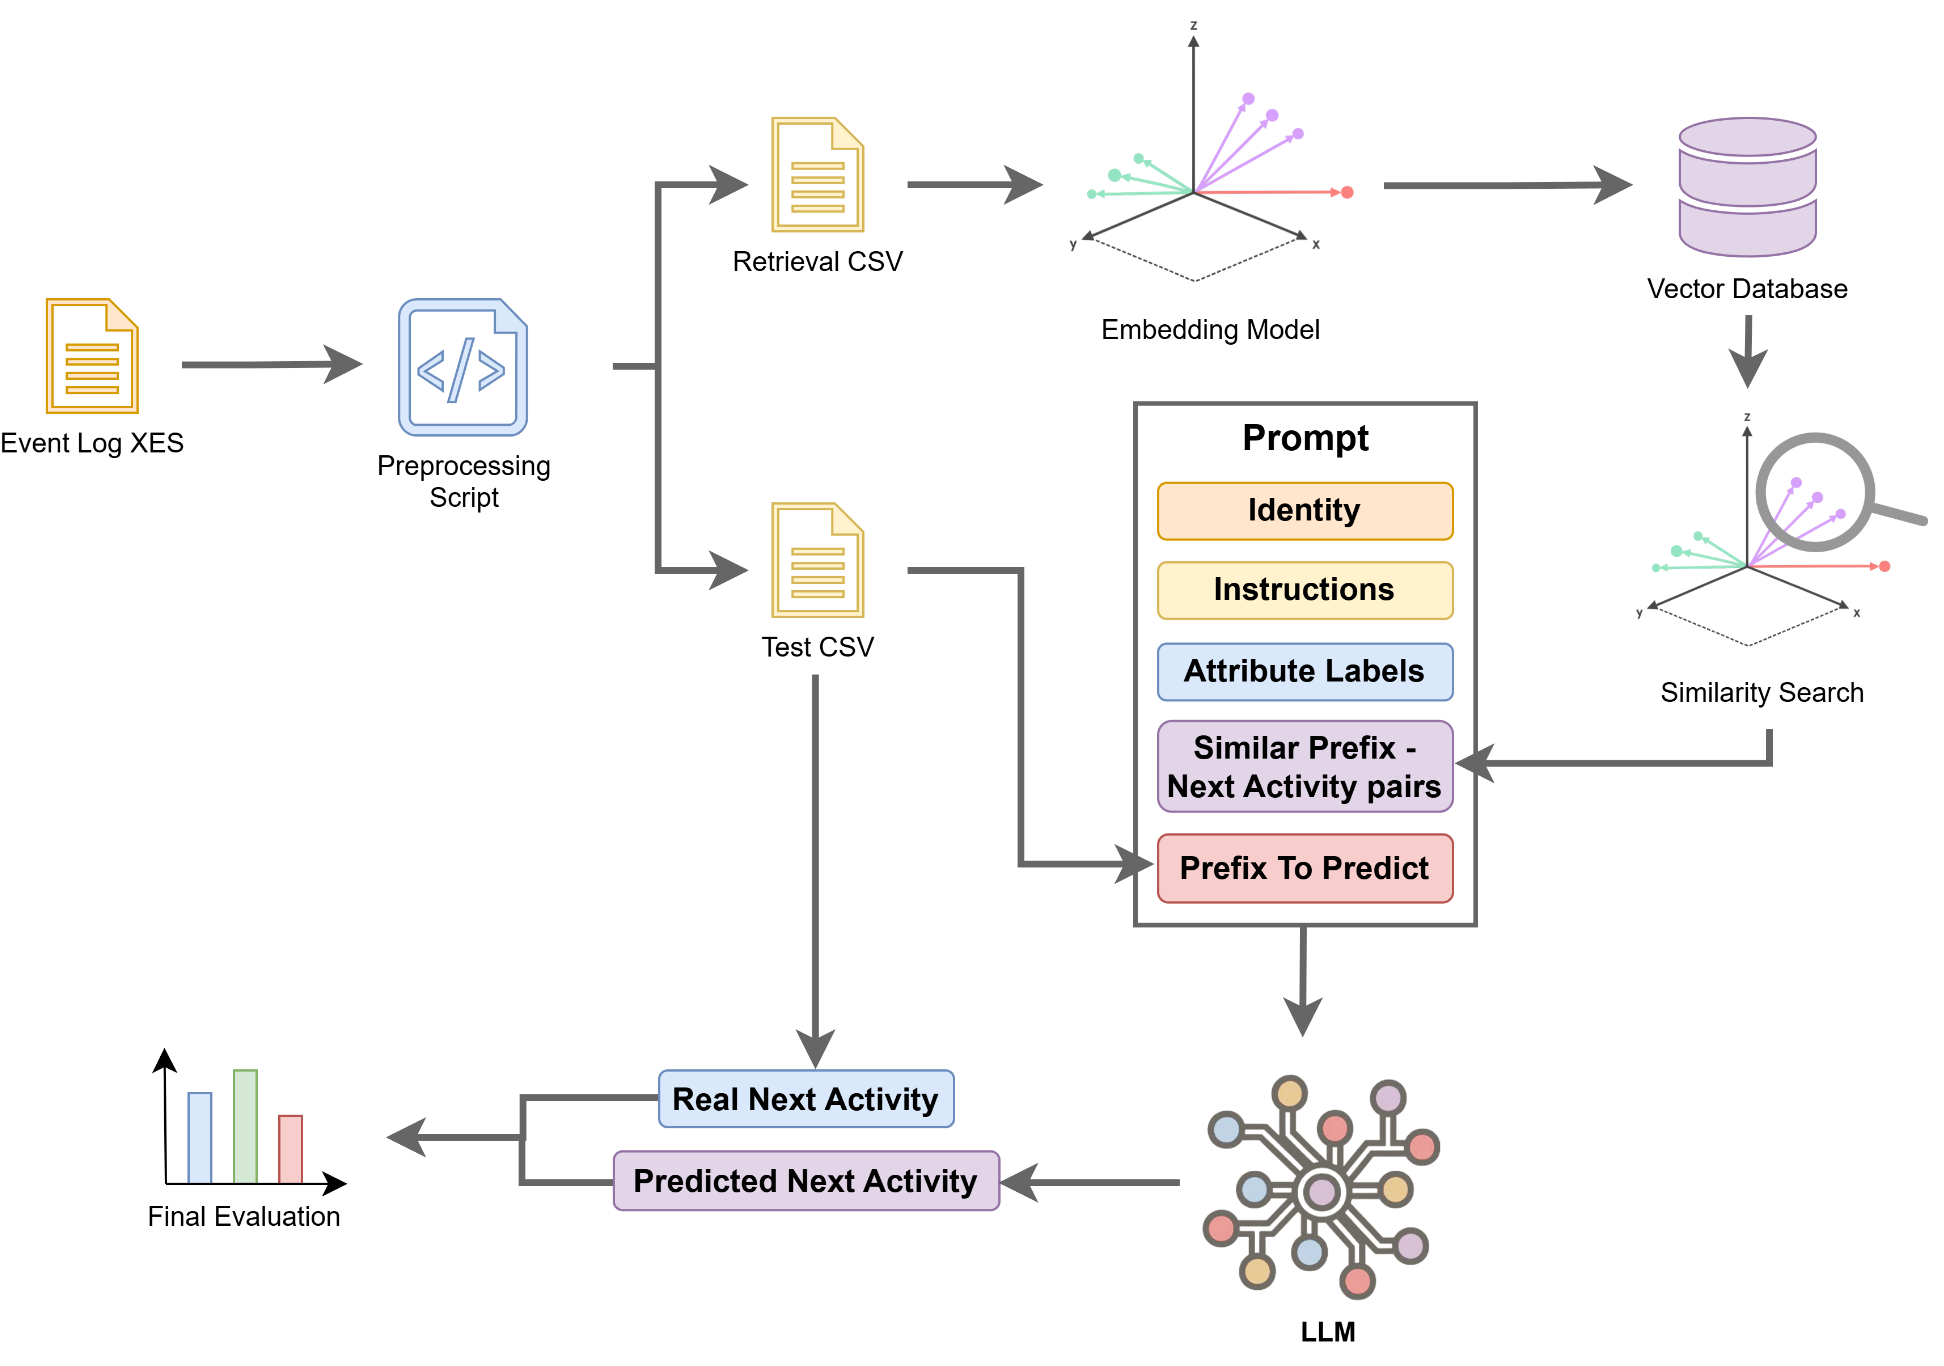
\includegraphics[width=\textwidth]{figures/pipeline_overview.png}
\caption{High-level overview of the full pipeline and evaluation flow}
\label{fig:full-pipeline-overview}
\end{figure}

\section{Data Preprocessing}
Preprocessing starts from the original event log stored in XES format and
converts it into a tabular representation in which each row corresponds to a
single event of a process execution. At this stage, only the basic information
required to reconstruct the event sequence of each case is preserved, namely
the execution identifier, the activity name, the timestamp, and the available
event-level attributes.

An initial cleaning step is then applied to remove records that are not
suitable for the prediction setting. When lifecycle information is available
in the log, only the events that indicate that an activity has been completed
are retained. This ensures that each activity is represented once as an actual
process step and prevents intermediate or auxiliary lifecycle transitions from
distorting the execution sequence.

\indent The next step restricts the set of attributes that are propagated to
the later stages. Trace-level attributes that describe the execution as a
whole are removed, with the exception of the trace identifier that is required
to group events into the same trace. In contrast, event-level attributes that
accompany each activity are preserved. This makes the dataset more consistent,
avoids redundant information, and ensures that subsequent processing focuses
mainly on the dynamic behavior of the process.

\indent After cleaning, events are grouped by trace and arranged in the
correct chronological order. This step is critical because next-activity
prediction assumes an accurate representation of the path followed so far by
each trace. For this reason, the sequence of events is reconstructed
according to the available timestamps and, where necessary, the original
appearance order is retained to resolve ties without altering the actual trace
structure.

\indent The outcome of this stage is not yet a learning-ready feature set,
but a clean, consistent, and chronologically organized body of data that can
support the subsequent construction of prefixes and prediction targets.

\paragraph{Example before and after preprocessing}\mbox{}\par\vspace{\baselineskip}

\begin{lstlisting}[
    style=xmlstyle,
    caption={Raw trace fragment from the original XES log},
    label={lst:raw-xes-fragment}
]
<event>
  <string key="lifecycle:transition" value="COMPLETE"/>
  <string key="concept:name" value="A_SUBMITTED"/>
  <date key="time:timestamp" value="2011-10-01T00:38:44.546+02:00"/>
</event>
<event>
  <string key="lifecycle:transition" value="COMPLETE"/>
  <string key="concept:name" value="A_PARTLYSUBMITTED"/>
  <date key="time:timestamp" value="2011-10-01T00:38:44.880+02:00"/>
</event>
<event>
  <string key="lifecycle:transition" value="SCHEDULE"/>
  <string key="concept:name" value="W_Completeren aanvraag"/>
  <date key="time:timestamp" value="2011-10-01T00:39:38.875+02:00"/>
</event>
<event>
  <string key="lifecycle:transition" value="START"/>
  <string key="concept:name" value="W_Completeren aanvraag"/>
  <date key="time:timestamp" value="2011-10-01T11:36:46.437+02:00"/>
</event>
<event>
  <string key="lifecycle:transition" value="COMPLETE"/>
  <string key="concept:name" value="A_ACCEPTED"/>
  <date key="time:timestamp" value="2011-10-01T11:42:43.308+02:00"/>
</event>
\end{lstlisting}

\begin{table}[H]
\centering
\caption{Dataframe after preprocessing}
\label{tab:preprocessed-dataframe}
\small
\begin{tabular}{llll}
\toprule
\textbf{trace\_id} & \textbf{activity} & \textbf{timestamp} & \textbf{lifecycle} \\
\midrule
173688 & A\_SUBMITTED & 2011-10-01 00:38:44.546+02:00 & COMPLETE \\
173688 & A\_PARTLYSUBMITTED & 2011-10-01 00:38:44.880+02:00 & COMPLETE \\
173688 & A\_PREACCEPTED & 2011-10-01 00:39:37.906+02:00 & COMPLETE \\
173688 & A\_ACCEPTED & 2011-10-01 11:42:43.308+02:00 & COMPLETE \\
\bottomrule
\end{tabular}
\end{table}

\noindent
The example illustrates an indicative trace fragment from the
original XES log and its corresponding form after preprocessing. In the raw
version, each event contains lifecycle information and timestamps, whereas
after preprocessing only completed activities and the core attributes required
by the later stages are retained.

\section{Feature Construction and Selection}
After preprocessing, each clean trace is transformed into a set of training
examples suitable for next-activity prediction. The key idea is that a
complete trace is not used as a single sample. Instead, it is decomposed into
multiple prefixes. Each prefix represents the execution state of the process
up to a specific point, while the target label is defined as the immediately
following activity. In this way, the original event log is converted into a
collection of prefix--target pairs that can be used both for retrieval and
for final prediction.

\indent Feature construction is based on two complementary sources of
information. The first is the \textit{control-flow}, namely the sequence of
activities that has already been executed in the trace. The second is the
\textit{data payload}, which contains the values of the attributes associated
with the individual events. In the proposed pipeline, these two aspects are
not encoded as a conventional numerical feature vector. Instead, they are
transformed into a structured textual representation, where the prefix
preserves the sequential activity structure while also including selected
attribute values from the most recent events.

\indent Formally, let a trace be denoted by
\[
\sigma = \langle e_1, e_2, \dots, e_n \rangle,
\]
where \(e_i\) is the \(i\)-th event of the case. For any eligible position
\(t < n\), the corresponding prefix is
\[
p_t = \langle e_1, e_2, \dots, e_t \rangle,
\]
and the prediction target is the activity of the immediately following event,
denoted by
\[
y_t = a_{t+1}.
\]

\indent The generation of prefixes is controlled by the \textit{base}
parameter, which defines the minimum length from which examples start to be
created. This avoids generating excessively short prefixes, which usually
contain limited information and are not sufficiently representative of the
actual state of the case. For each eligible point in a trace, the sequence of
activities up to that point is used as the observed history, while the
immediately following activity is used as the correct answer to be predicted.

\indent The \textit{gap} parameter determines the spacing between
consecutively generated prefixes. Instead of creating a new example after
every next event, the pipeline can construct prefixes at sparser intervals.
This reduces the density of almost identical examples and controls the size of
the resulting dataset without removing the essential ordering information. The
use of gap-based prefix generation follows a design logic already discussed in
predictive process monitoring literature~\ieeecite{bib:dfm2015}{1}. In the
final evaluation, this parameter is treated as one of the main experimental
levers because it directly affects how finely the evolution of each trace is
observed.

\indent Taken together, \textit{base} and \textit{gap} define the set of
eligible prefix lengths. If \(\textit{base}=b\) and \(\textit{gap}=g\), these
lengths can be written as
\[
\ell_k = b + kg, \qquad k = 0,1,2,\dots,
\]
subject to \(\ell_k < n\), where \(n\) is the length of the trace. The
generated examples therefore take the form
\[
(p_{\ell_k}, y_{\ell_k}).
\]
This parameterization offers a simple way to control dataset granularity.
Larger gap values reduce the number of generated examples and therefore help
limit the size of the final dataset, but they also make the observation of the
trace evolution coarser, since some intermediate states are no longer
explicitly represented.

\indent Particularly important is the \textit{m} parameter, which defines how
much recent attribute information is retained within the prefix. In the
present implementation, the full activity sequence remains visible, but
detailed \textit{value blocks} are preserved only for the last \(m\) events.
As a result, the model has access to the complete control-flow history, while
only a limited and recent attribute context is kept in explicit form. This
design is aligned with the literature on \textit{last state encoding}, where
the latest available snapshot of dynamic attributes is preserved and the
method can be extended to \textit{last \(m\) states}~\ieeecite{bib:teinemaa2018}{2}.
In this pipeline, the same idea is adapted into a textual representation by
keeping only the last \(m\) value blocks within each prefix.

\indent If a prefix ends at position \(t\), the control-flow history remains
fully visible, while explicit attribute-value blocks are retained only for the
events whose indices belong to the set
\[
\{i \mid \max(1, t-m+1) \leq i \leq t\}.
\]
Thus, the representation keeps the full sequential history but restricts the
detailed data payload to the most recent \(m\) events.

\indent These values are not stored as isolated independent fields. Instead,
they form a snapshot of the most recently available attribute state up to the
examined point. In other words, each new event updates the current attribute
picture, and only the most recent relevant snapshots remain visible in the
final representation. In addition, attribute names are compacted into shorter
identifiers so that the prefix remains concise and usable in the later stages
of the pipeline without losing its informational content.

\indent Finally, deduplication is applied so that the same prefix--target pair
is not stored multiple times. This reduces redundant information and leads to
a more coherent collection of examples. The outcome of this stage is an
organized set of textual prefixes that captures both the execution path of
each trace and the most critical recent attribute context, as demonstrated in
Listing~\ref{lst:indicative-prefix-representation}.

\vspace{\baselineskip}

\begin{lstlisting}[
    basicstyle=\ttfamily\footnotesize,
    columns=fullflexible,
    keepspaces=true,
    breaklines=false,
    showstringspaces=false,
    frame=none,
    xleftmargin=0pt,
    xrightmargin=0pt,
    aboveskip=0pt,
    belowskip=0pt,
    caption={Indicative prefix representation},
    label={lst:indicative-prefix-representation}
]
event_A {Values},event_B {Values}
event_A,event_B,event_C {Values},event_D {Values},event_E {Values}
event_A,event_B,event_C,event_D,event_E,event_F {Values},event_G {Values},event_H {Values}
...
\end{lstlisting}

\par\noindent
The above example shows successive prefixes following the same representation
logic. For \textit{base}=1, the first prefix is produced once the first two
events have been observed. For \textit{gap}=3, each subsequent prefix is
extended by three new events. Finally, for \textit{m}=3, detailed
\textit{Values} are retained only for the three most recent events, whereas
older activities remain visible only as part of the \textit{control-flow}.

\section{Split Strategy}
After feature construction, the pipeline can create the retrieval and test
collections in two different ways. The difference lies in \textit{when} the
split is applied and in \textit{which unit} is being separated. In both cases,
deduplication follows the same internal key used by the implementation,
namely the control-flow representation of the prefix together with its target
label.

\subsection{Prefix Level}
In the first mode, the full event log is processed as a single body of data.
All traces are first converted into one global table of prefix--target pairs.
At this stage, global deduplication is already active, so repeated
control-flow-and-label combinations are removed before the final split is
created. As a result, the full prefix table contains only one retained copy of
each unique training example under the implemented deduplication rule.

\indent Once this globally deduplicated table has been produced, the split is
applied directly at the prefix level. In the current implementation, 30\% of
the rows are sampled from the table to form the test set, while the remaining
70\% form the retrieval set. In this configuration, the unit of separation is
therefore the individual prefix row rather than the original trace. Since the
split happens after all prefixes have already been generated, prefixes
originating from the same original trace may end up on both sides, provided
that they are not removed by the global deduplication step.

\indent This mode is retrieval-oriented. It evaluates the system in a setting
where the retrieval collection and the test collection are both derived from
the same globally generated prefix space, but exact duplicates according to
the deduplication key are removed before row sampling takes place.

\subsection{Trace Level}
In the second mode, the split is applied before prefix generation. The
original XES log is first divided into two valid XES files at the trace level:
a training-side file and a test-side file. In the current implementation,
70\% of the traces are assigned to the retrieval side and the remaining 30\%
to the test side. The traces are ordered chronologically according to their
end timestamps, and the earlier portion is assigned to retrieval while the
later portion is assigned to testing. In this way, the retrieval side is
built from earlier completed cases and the test side from later completed
cases.

\indent After these split files are created, each side is processed through the
same preprocessing and prefix-construction pipeline. At this point, the trace-
level mode can be used in two variants: without cross-split deduplication and
with cross-split deduplication. In the non-deduplicated variant, the
training-side XES file is transformed into the retrieval CSV and the test-side
XES file is transformed into the test CSV independently, without any shared
deduplication state across the two sides. As a result, the same
control-flow-and-label combination may appear in both retrieval and test if it
is generated from different traces.

\indent In the deduplicated variant, the same chronological trace split is
kept, but a shared global deduplication state is used across retrieval and
test during prefix generation. This means that once a
control-flow-and-label combination has already been retained on the retrieval
side, the same combination is not stored again on the test side. Because the
retrieval side is processed first, the retained unique copy remains in
retrieval and is excluded from the later test collection.

\begin{figure}[H]
\centering
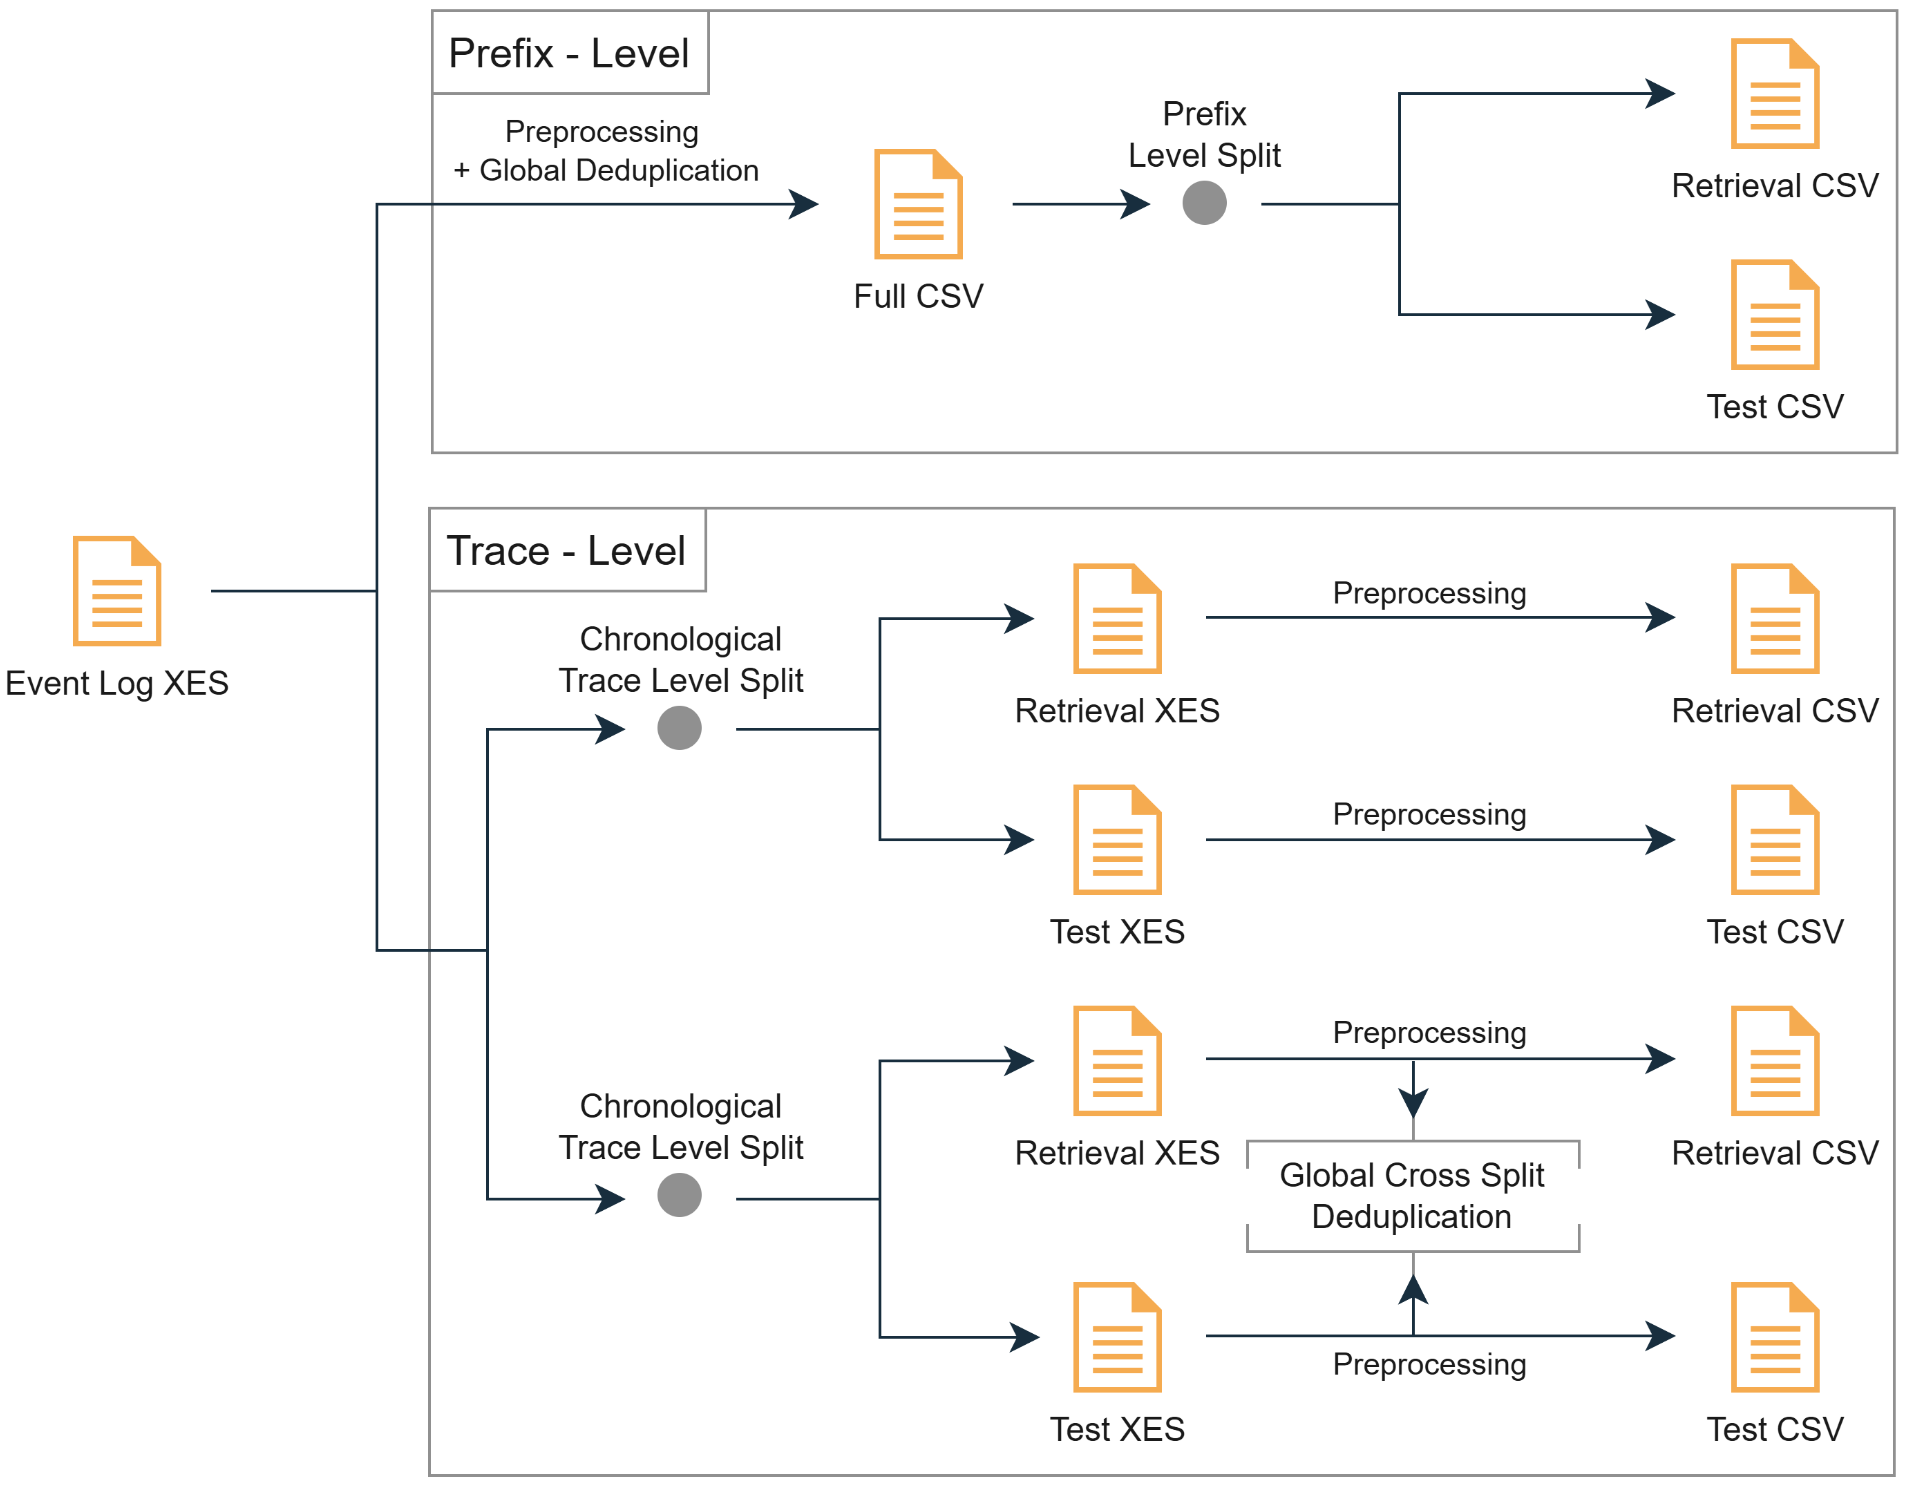
\includegraphics[width=0.96\textwidth]{figures/split_strategy_pipeline.png}
\caption{Split strategy pipeline}
\label{fig:split-strategy-pipeline}
\end{figure}

\section{Retrieval Layer}
Once the retrieval and test CSV files have been created, the next stage of the
pipeline builds a searchable memory over the historical prefixes contained in
the retrieval set. Each row of the retrieval CSV consists of a textual prefix
and its corresponding next-activity label. The prefix is treated as the
retrievable object, while the label is stored together with it so that, once a
similar historical example is found, its known continuation can be passed to
the prediction stage as contextual evidence.

\indent To make this search possible, each retrieval prefix is transformed into
a dense vector representation through an embedding model. In this way,
prefixes that are similar in sequential structure and recent attribute context
are mapped to nearby points in the vector space. After all retrieval prefixes
have been encoded, their vector representations are stored together with the
original textual prefix and the associated target label. As a result, the
retrieval layer preserves both the compact numerical representation needed for
similarity search and the original symbolic information needed for prompt
construction.

\indent During evaluation, each query prefix taken from the test CSV is encoded
with the same embedding model. The resulting query vector is then compared
against the stored retrieval vectors through similarity search, using a
cosine-based comparison in the embedding space. The pipeline
returns the top \(k\) most similar historical prefixes, where \(k\) is a
configurable parameter of the experiment. Each retrieved item therefore
contains three elements: the historical prefix itself, its known next-activity
label, and its similarity score with respect to the query prefix. The role of
this step is to provide a compact set of highly relevant past examples rather
than the full retrieval collection.

\indent An optional second ranking step can also be applied after the initial
vector search. In this variant, a larger candidate pool is first collected by
similarity search and then reordered according to a learned pairwise relevance
criterion between the query prefix and each candidate prefix. The final top
\(k\) examples are then selected from this reordered list. Whether this second
ranking stage is used or not, the retrieval layer always produces the same
type of output: a small ordered set of historical prefix--label examples that
are passed to the prompt construction stage.

\section{Prompt Construction}
After the retrieval stage, the selected historical examples must be converted
into a form that can be directly consumed by the language model. For this
reason, the pipeline does not pass the query prefix alone. Instead, it builds
a structured prompt that combines task instructions, contextual information,
and the prefix whose next activity must be predicted.

\indent The prompt is organized into a small number of clearly separated
blocks, as shown in Figure~\ref{fig:vector-database-prompt-context}. First, an
\textit{identity} block specifies that the model acts as a
process-mining assistant specialized in predictive monitoring. Second, an
\textit{instruction} block defines the task itself, namely to predict the next
activity immediately after the last activity of the given prefix and to return
the answer in a strictly controlled format. Third, the prompt may include an
\textit{attribute legend}, which explains the compact attribute identifiers
used in the textual prefix representation. Finally, the prompt includes the
retrieved historical examples, each represented as a past prefix together with
its known next activity.

\indent After these contextual sections, the target prefix is appended as the
final query to be solved by the model. In this way, the model receives both
the current process state and a compact memory of similar historical
continuations. The retrieved examples therefore function as in-context
evidence, while the query prefix defines the specific prediction instance of
interest.

\indent Two prompt variants are used in the experiments. The first is a general
retrieval-based prompt, which instructs the model to reason from the retrieved
past traces and the values of the most recent events. The second follows the
same overall structure, but places stronger emphasis on the most recent
attribute values retained by the \textit{last-\(m\)} representation. The two
variants therefore differ less in layout than in the weight they assign to the
latest visible attribute context when predicting the continuation of the
prefix.

\begin{figure}[H]
\centering
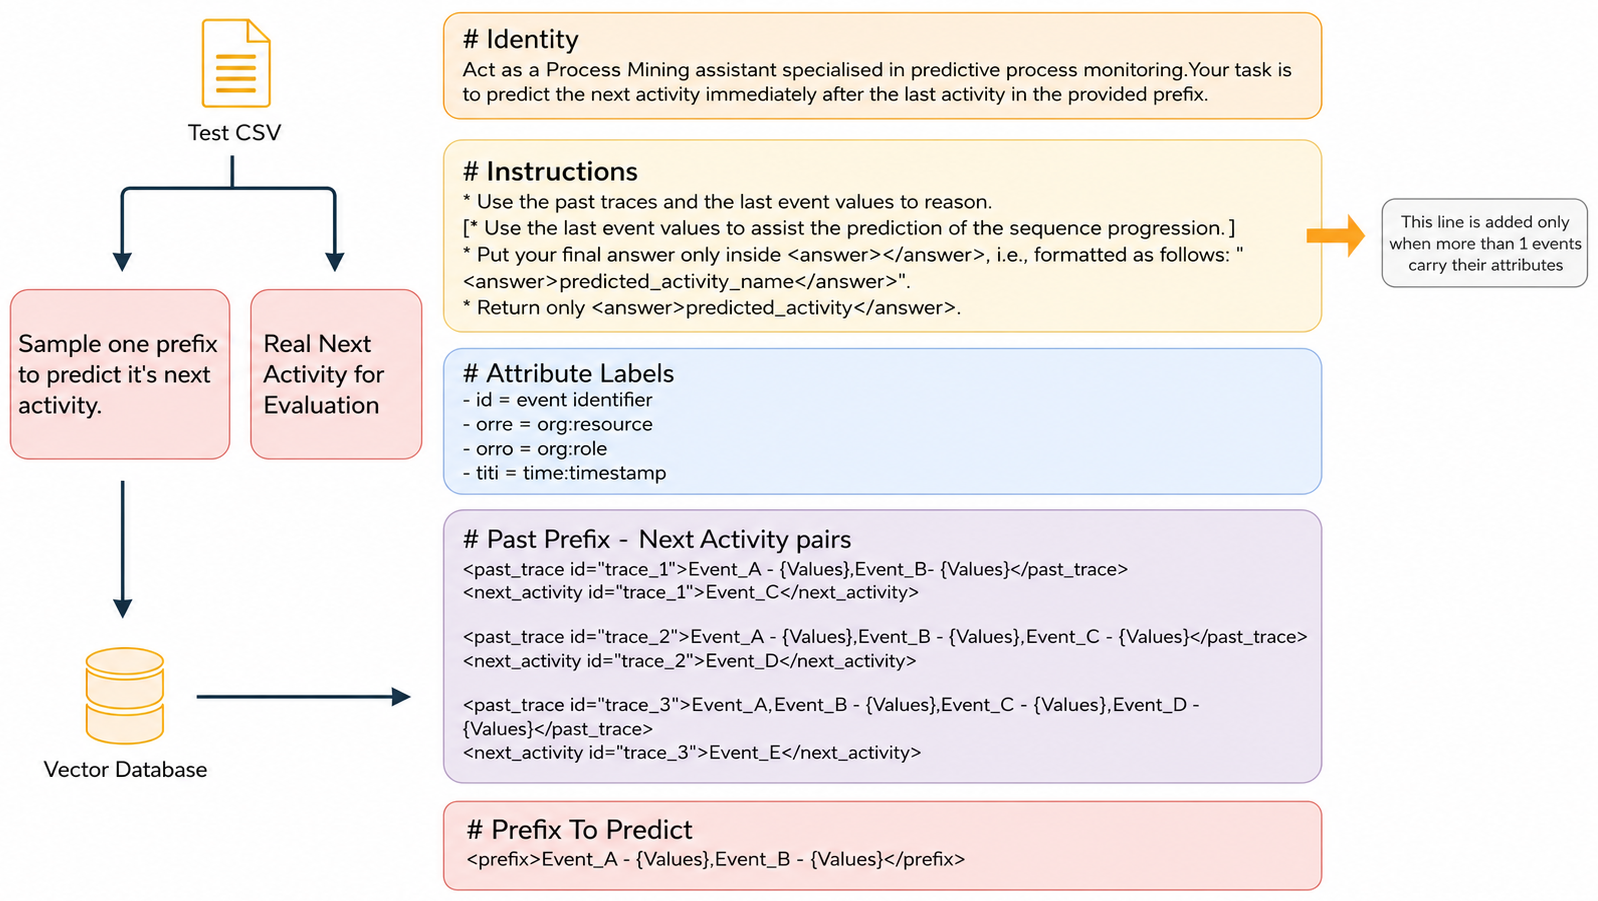
\includegraphics[width=0.92\textwidth]{figures/prompt_42_replacement.png}
\caption{Vector database context within prompt construction}
\label{fig:vector-database-prompt-context}
\end{figure}

\section{Prediction Flow}
Once the final prompt has been assembled, it is submitted to the selected
language model in order to generate the next-activity prediction for the
query prefix. At this stage, the prompt already contains the task
instructions, the retrieved historical examples, the attribute legend when
available, and the prefix to be predicted. The role of the model is therefore
not to reconstruct the context, but to infer the most plausible activity that
should follow the current execution state.

\indent To make the output interpretable and machine-readable, the model is
asked to return its final answer in a strictly constrained form, namely inside
\texttt{<answer></answer>} tags. In this way, the prediction stage does not
depend on free-form generated text, but on an explicitly delimited output
segment that can be isolated reliably even when the model produces additional
reasoning or explanatory material. The generation itself is performed in a
deterministic setting, so that the variability introduced by sampling is
minimized during evaluation.

\indent After the model response is received, the pipeline extracts the
content enclosed within the \texttt{<answer></answer>} tags and treats this
text as the predicted next activity. The extracted label is then normalized so
that formatting differences do not affect the comparison with the ground
truth. In particular, surrounding spaces and quotation marks are removed, and
the label is converted to a standardized lowercase form before evaluation.

\indent If the response does not contain a valid answer block, or if the
extracted content corresponds to an empty or null-like output, the prediction
is treated as invalid and is not counted as a successful evaluated case. Only
responses that can be parsed into a valid activity label are retained as final
predictions. For each accepted case, the normalized predicted label is stored
together with the corresponding ground-truth next activity of the test row.

\indent The final result of this stage is therefore a collection of
prediction--target pairs, one for each valid query prefix processed during the
evaluation run. These pairs form the direct input to the metric computation
stage, where correctness is assessed and aggregate performance values such as
accuracy, macro-precision, macro-recall, and macro-\(F_1\) are calculated.

\blankpage
